\chapter{Context and Related Work}
\label{cha:related_work}
\minitoc

\section{Global Warming and ICT Role}
Global warming is one of the most critical environmental issues of our day \cite{houghton2005global}. Global warming is the effect of human activities on the climate, mainly the burning of fossil fuels (coal, oil, and gas) and large-scale deforestation \cite{houghton2005global}. Both activities have grown immensely since the industrial revolution. The burning of fossil fuels process results in greenhouse gas emissions \cite{olabi2022renewable}. Today, fossil fuels are one of the world's main sources of energy production, helping to emit more and more GHG \cite{olabi2022renewable}. GHG stays in the atmosphere creating a layer as a blanket over the planet's surface. Without this blanket, the Earth can balance the radiation energy from the sun and the thermal radiation from the Earth to space \cite{houghton2005global}. However, this human-generated blanket imposes a barrier to the thermal radiation from the Earth, letting it into the atmosphere and heating the planet, working as a greenhouse. All this process works as a greenhouse which is the reason for the name greenhouse gas \cite{houghton2005global}.

This situation brings us to United Nations Climate Change Conference (COP21) in Paris, France, on 12 December 2015. At this conference, 196 signed the Paris Agreement aiming to \cite{nations_paris_nodate}:
\begin{enumerate}
    \item Reduce global greenhouse gas emissions substantially, limiting the global temperature increase in this century to 2\degree C while pursuing measures to limit the growth even further to 1.5\degree C;
    \item Review countries’ commitments every five years (through the Nationally Determined Contribution, or NDC);
    \item Provide financing to developing countries to mitigate climate change, strengthen resilience, and enhance their abilities to adapt to climate impacts. 
\end{enumerate}

These are ambitious but necessary objectives. Since then, countries and organizations have proposed several actions and pledges. However, a recent report indicates that the actual world's effort is not enough \cite{tracker2022projections}. Figure \ref{fig:ghg_cat} shows GHG emission and temperature estimations. We could see that there is a small reduction in emissions increase tendency. Nevertheless, this figure estimates that real-world actions based on current policies will lead to an increase of somewhere between 2.6 and 2.9\degree C by 2100. This estimation is well above the 1.5\degree C pursued by the Paris Agreement. Considering the targets proposed by the countries through NDC, the temperature will be around 2.4\degree C. In a scenario based on NDC targets and submitted and binding long-term targets, the prediction is a temperature of 2\degree C by 2100, the limit proposed by the Paris Agreement. The report forecasts an optimistic scenario analyzing the effect of net zero emissions targets of about 140 countries that are adopted or under discussion. Even in this optimistic scenario, the estimated temperature would be 1.8\degree C. The situation tends to be even worst with the gold rush for gas \cite{tracker2022massive}. The report indicates that in 2022 we arrived at 1.2\degree C warming \cite{tracker2022projections}.

\begin{figure}[!htb]
    \centering
    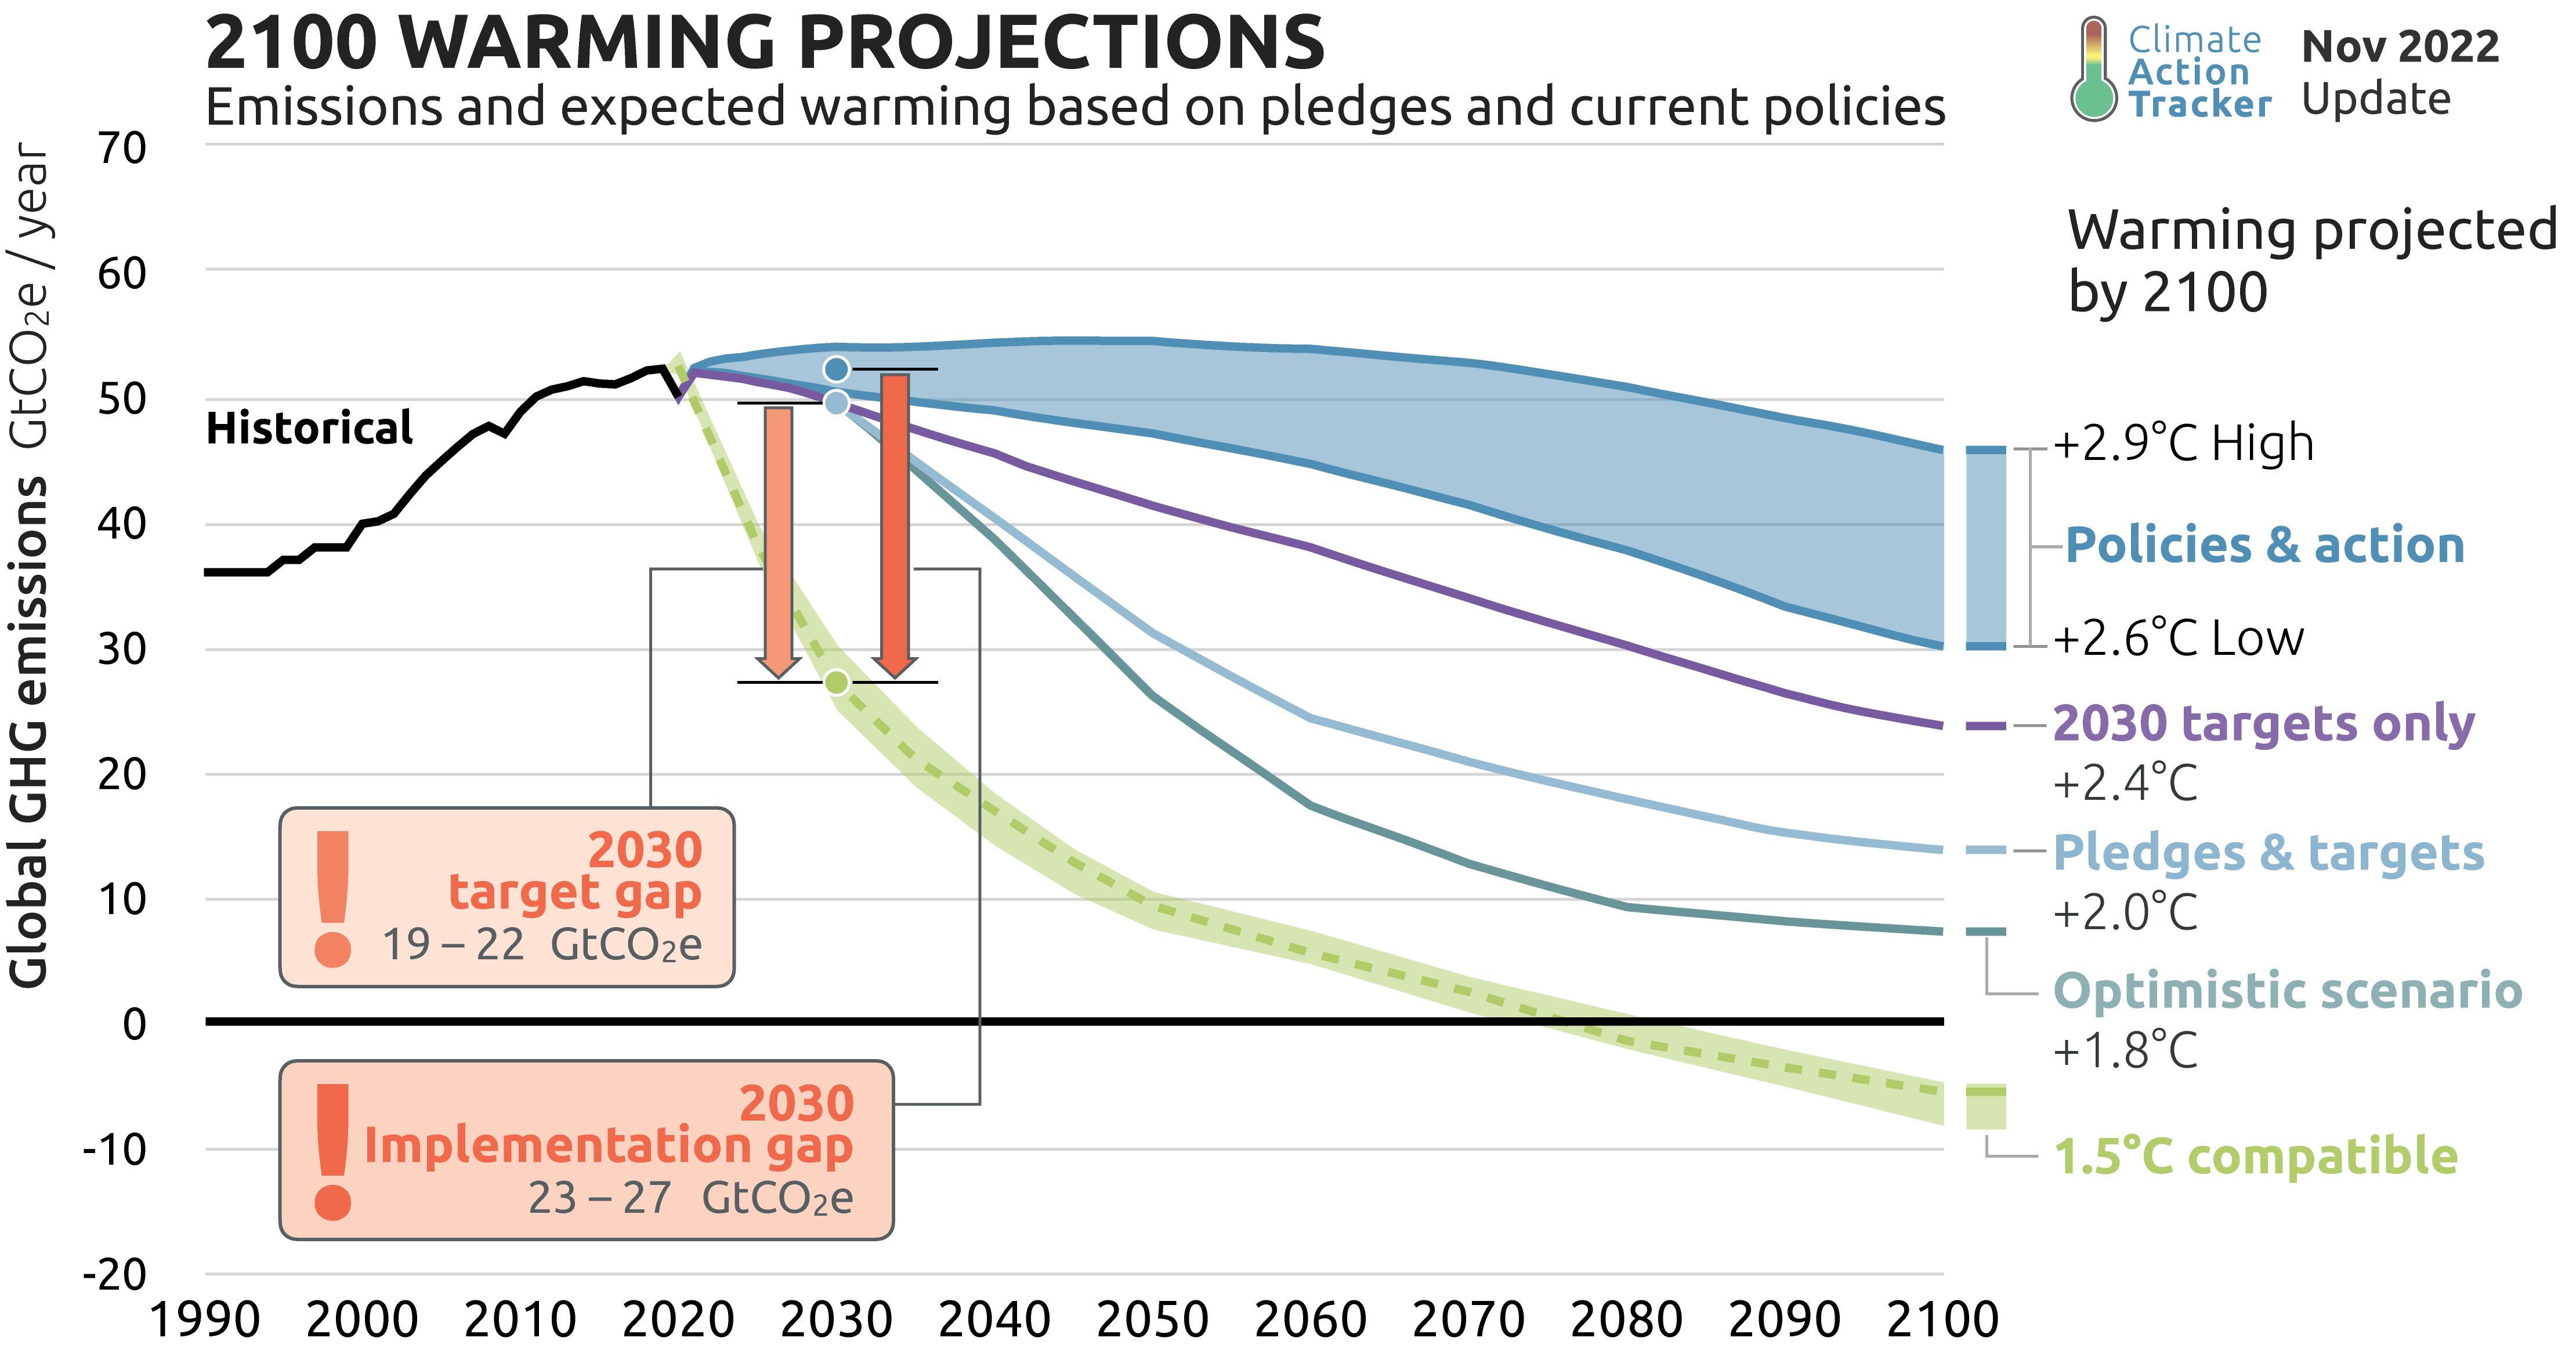
\includegraphics[scale=0.09]{Images/Related_works/Emissions_2022-11.png}
    \caption{Estimated global GHG emissions \cite{tracker2022projections}.}
    \label{fig:ghg_cat}
\end{figure}

We have started to feel the impacts of global warming on humanity, such as heatwaves, droughts, and floods, impacting flora and fauna directly \cite{masson2018global, change2022threat}. In a cascade effect, this increases food and water insecurity worldwide \cite{change2022threat, doi:10.1126/science.1239402}. Also, high temperatures increase mortality, impact labor productivity, impair learning, increase adverse pregnancy outcomes possibility, increase conflict, hate speech, migration, and infectious disease spread \cite{lenton2023quantifying}. Therefore, an increase of the temperature by 2.7\degree C as forecasted would impact one-third (22–39\%) of the world's population by 2100 \cite{lenton2023quantifying}. Climate change has already impacted around 9\% of people (>600 million) \cite{lenton2023quantifying}. Reducing global warming from 2.7 to 1.5\degree C results in a $\sim$5-fold decrease in the population exposed to unprecedented heat (mean annual temperature $\geq$29\degree C) \cite{lenton2023quantifying}. Thus, all sectors must reduce their GHG emissions as much as possible.

Information and Communication Technology is one of these sectors which has accelerated growth in the last 70 years. Unesco defines ICT as \cite{unesco2009guide}:

\begin{quote}
    ``Information and communication technologies (ICT) is defined as a diverse set of technological tools and resources used to transmit, store, create, share or exchange information. These technological tools and resources include computers, the Internet (websites, blogs, and emails), live broadcasting technologies (radio, television, and webcasting), recorded broadcasting technologies (podcasting, audio and, video players, and storage devices), and telephony (fixed or mobile, satellite, visio/video-conferencing, etc.).''
\end{quote}

Regarding the ICT role in GHG emissions, the global share is around 1.8\%-2.8\%, or 2.1\%-3.9\% considering the supply chain pathways in 2020 \cite{freitag2021climate}. The situation tends to get even worst, driven by the boom in Internet-connected devices. A Cisco report indicates that the Internet had 3.9 billion users in 2018 \cite{cisco2020cisco}. The same report predicts an increase to 5.3 billion in 2023 (66 percent of the global population). Also, they predicted 3.6 networked devices per capita in 2023, up from 2.4 networked devices per capita in 2018. However, International Telecommunication Union (ITU), a United Nations specialized agency for ICTs, indicates that we arrived at 5.3 billion connected users in 2022 due to the COVID-19 pandemic \cite{ITU2022}. But will the growth in internet users increase GHG emissions? Andrae and Edler \cite{andrae2015global} and Belkhir and Elmeligi \cite{belkhir2018assessing} agree that this growth could lead to an increase in GHG emissions. Figure \ref{fig:projections_ICT} shows the predictions of both works.

\begin{figure}[!htb]
    \centering
    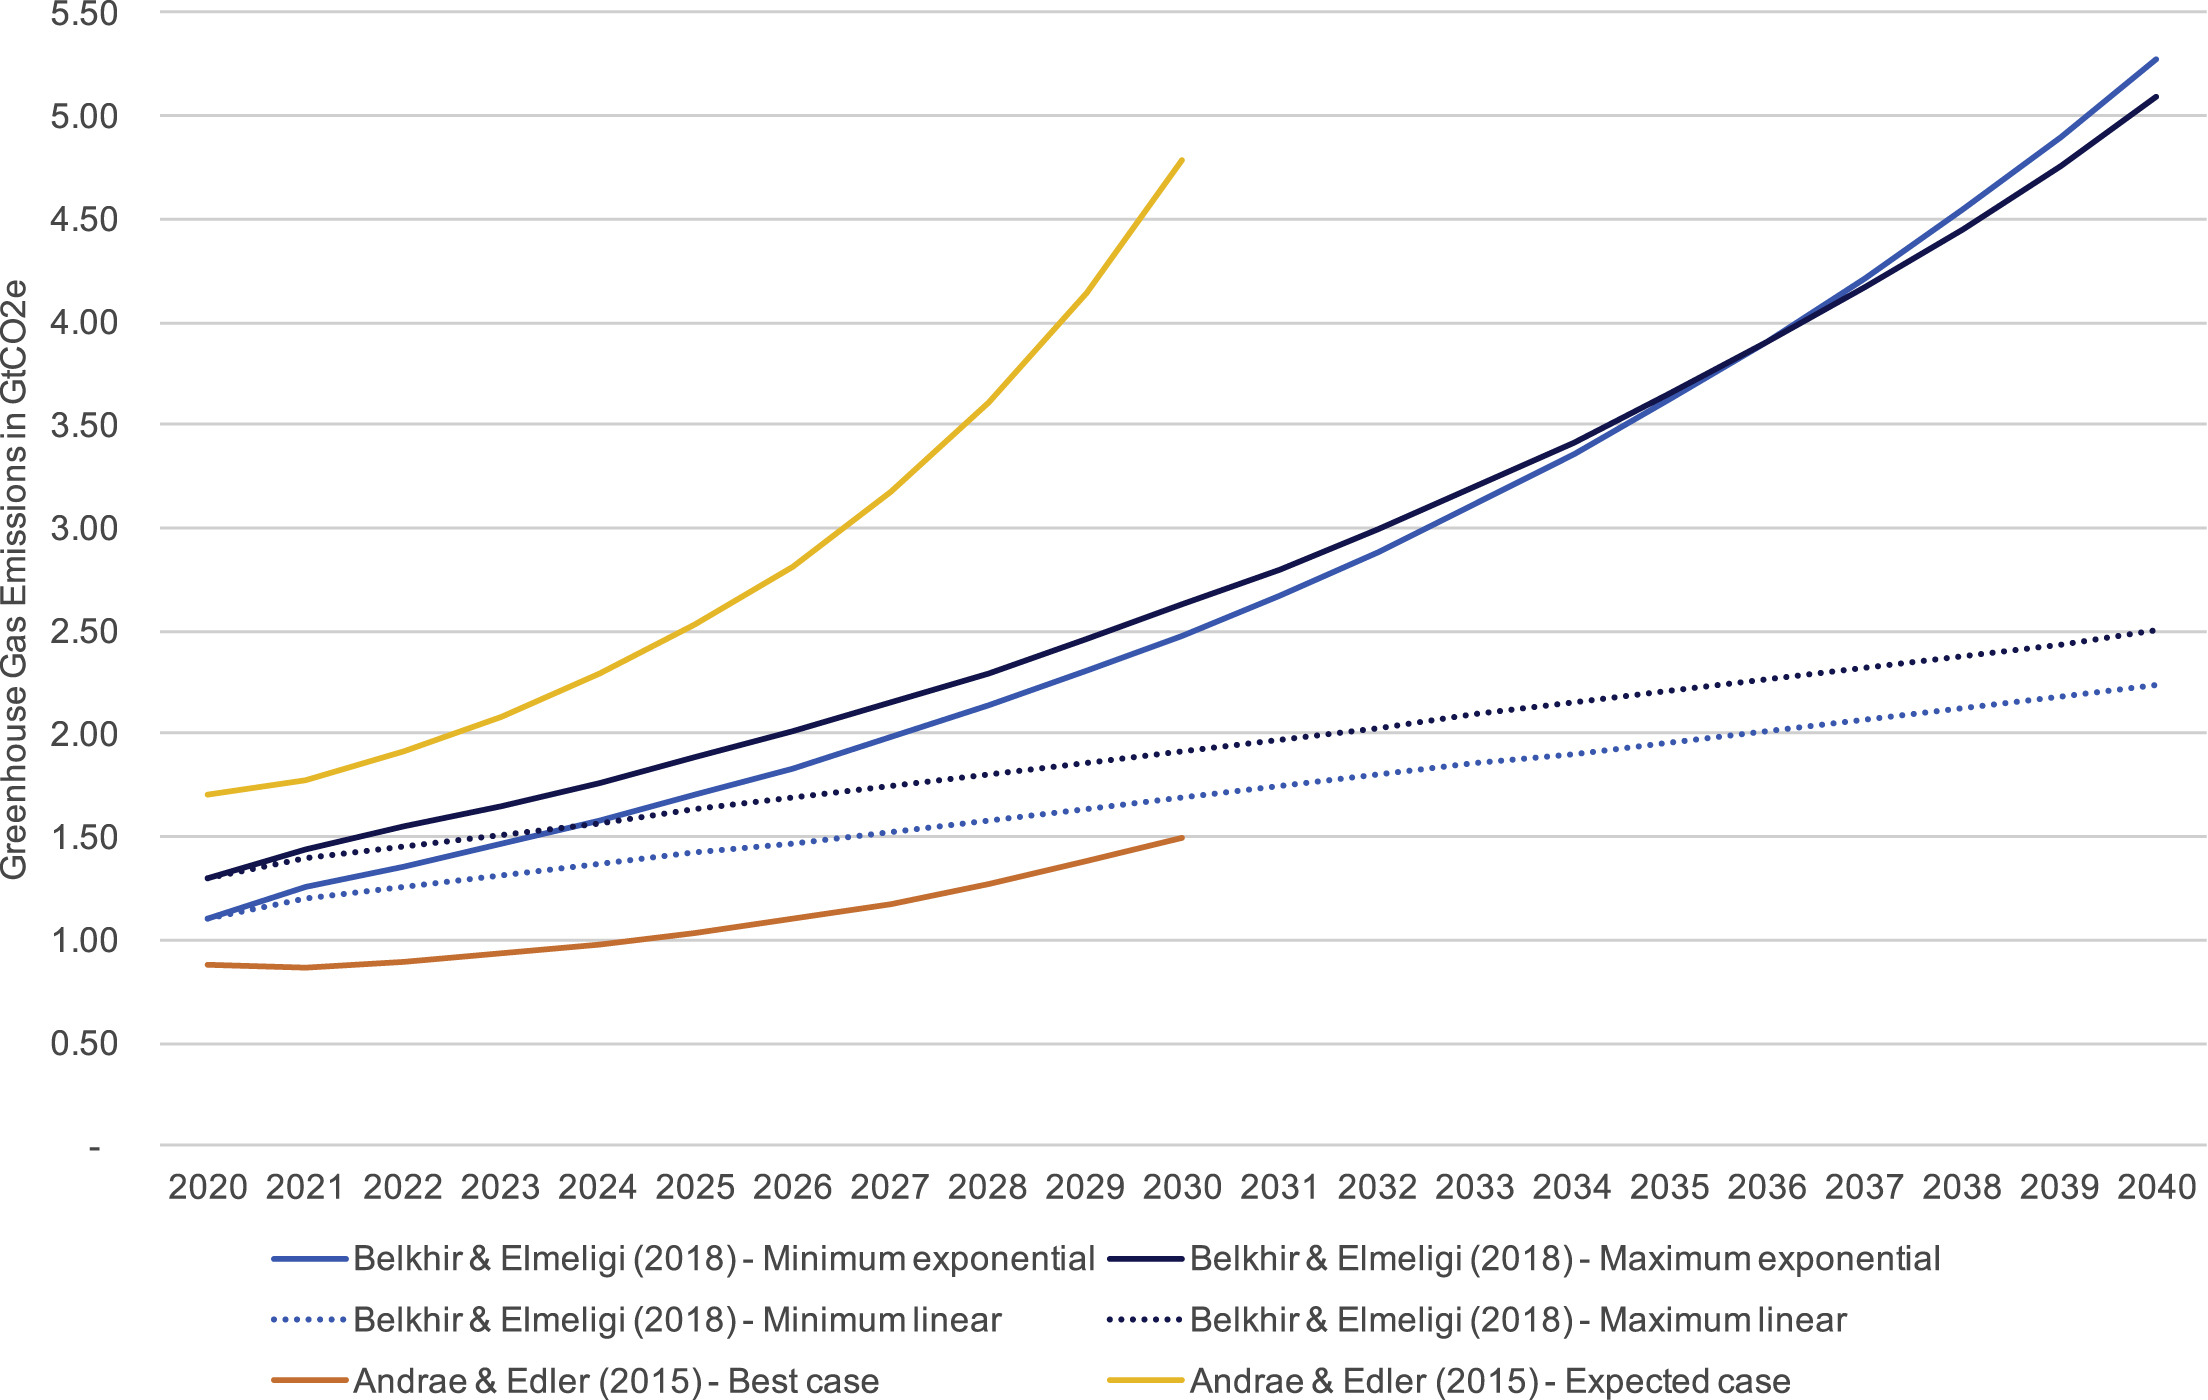
\includegraphics[scale=1]{Images/Related_works/gr4_lrg.jpg}
    \caption{Projections of ICT's GHG emissions from 2020 \cite{freitag2021climate}.}
    \label{fig:projections_ICT}
\end{figure}

This figure illustrates the contraction in the Paris Agreement demand and the predictions about usage in the ICT sector. In all forecasts of Figure \ref{fig:projections_ICT}, the tendency is emissions growth. However, ICT needs to reduce its emissions drastically. Figure \ref{fig:stable_emissions_ICT} illustrates the carbon emission share if the ICT stays at the same level as 2020 and the other sectors decrease their emissions. Without changes, ICT would have 35.1\% of global emissions in 2050. So, ICT must move towards reducing its emissions. Figure \ref{fig:estimations_ICT} presents the estimations of ICT's GHG emissions for 2015 and 2020 from different authors. This figure breaks down these emissions into different components. One of them, with a good share in some cases, is Data centers. IBM defines the data center as ``A data center is a physical room, building or facility that houses IT infrastructure for building, running, and delivering applications and services, and for storing and managing the data associated with those applications and services'' \cite{datacenterIBM}. The International Energy Agency (IEA) defines data center as \cite{centres2022data}:
\begin{quote}
    ``Data centers are facilities used to house networked computer servers that store, process and distribute large amounts of data. They use energy to power both the IT hardware (e.g., servers, drives, and network devices) and the supporting infrastructure (e.g., cooling equipment).''
\end{quote}

\begin{figure}[!htb]
    \centering
    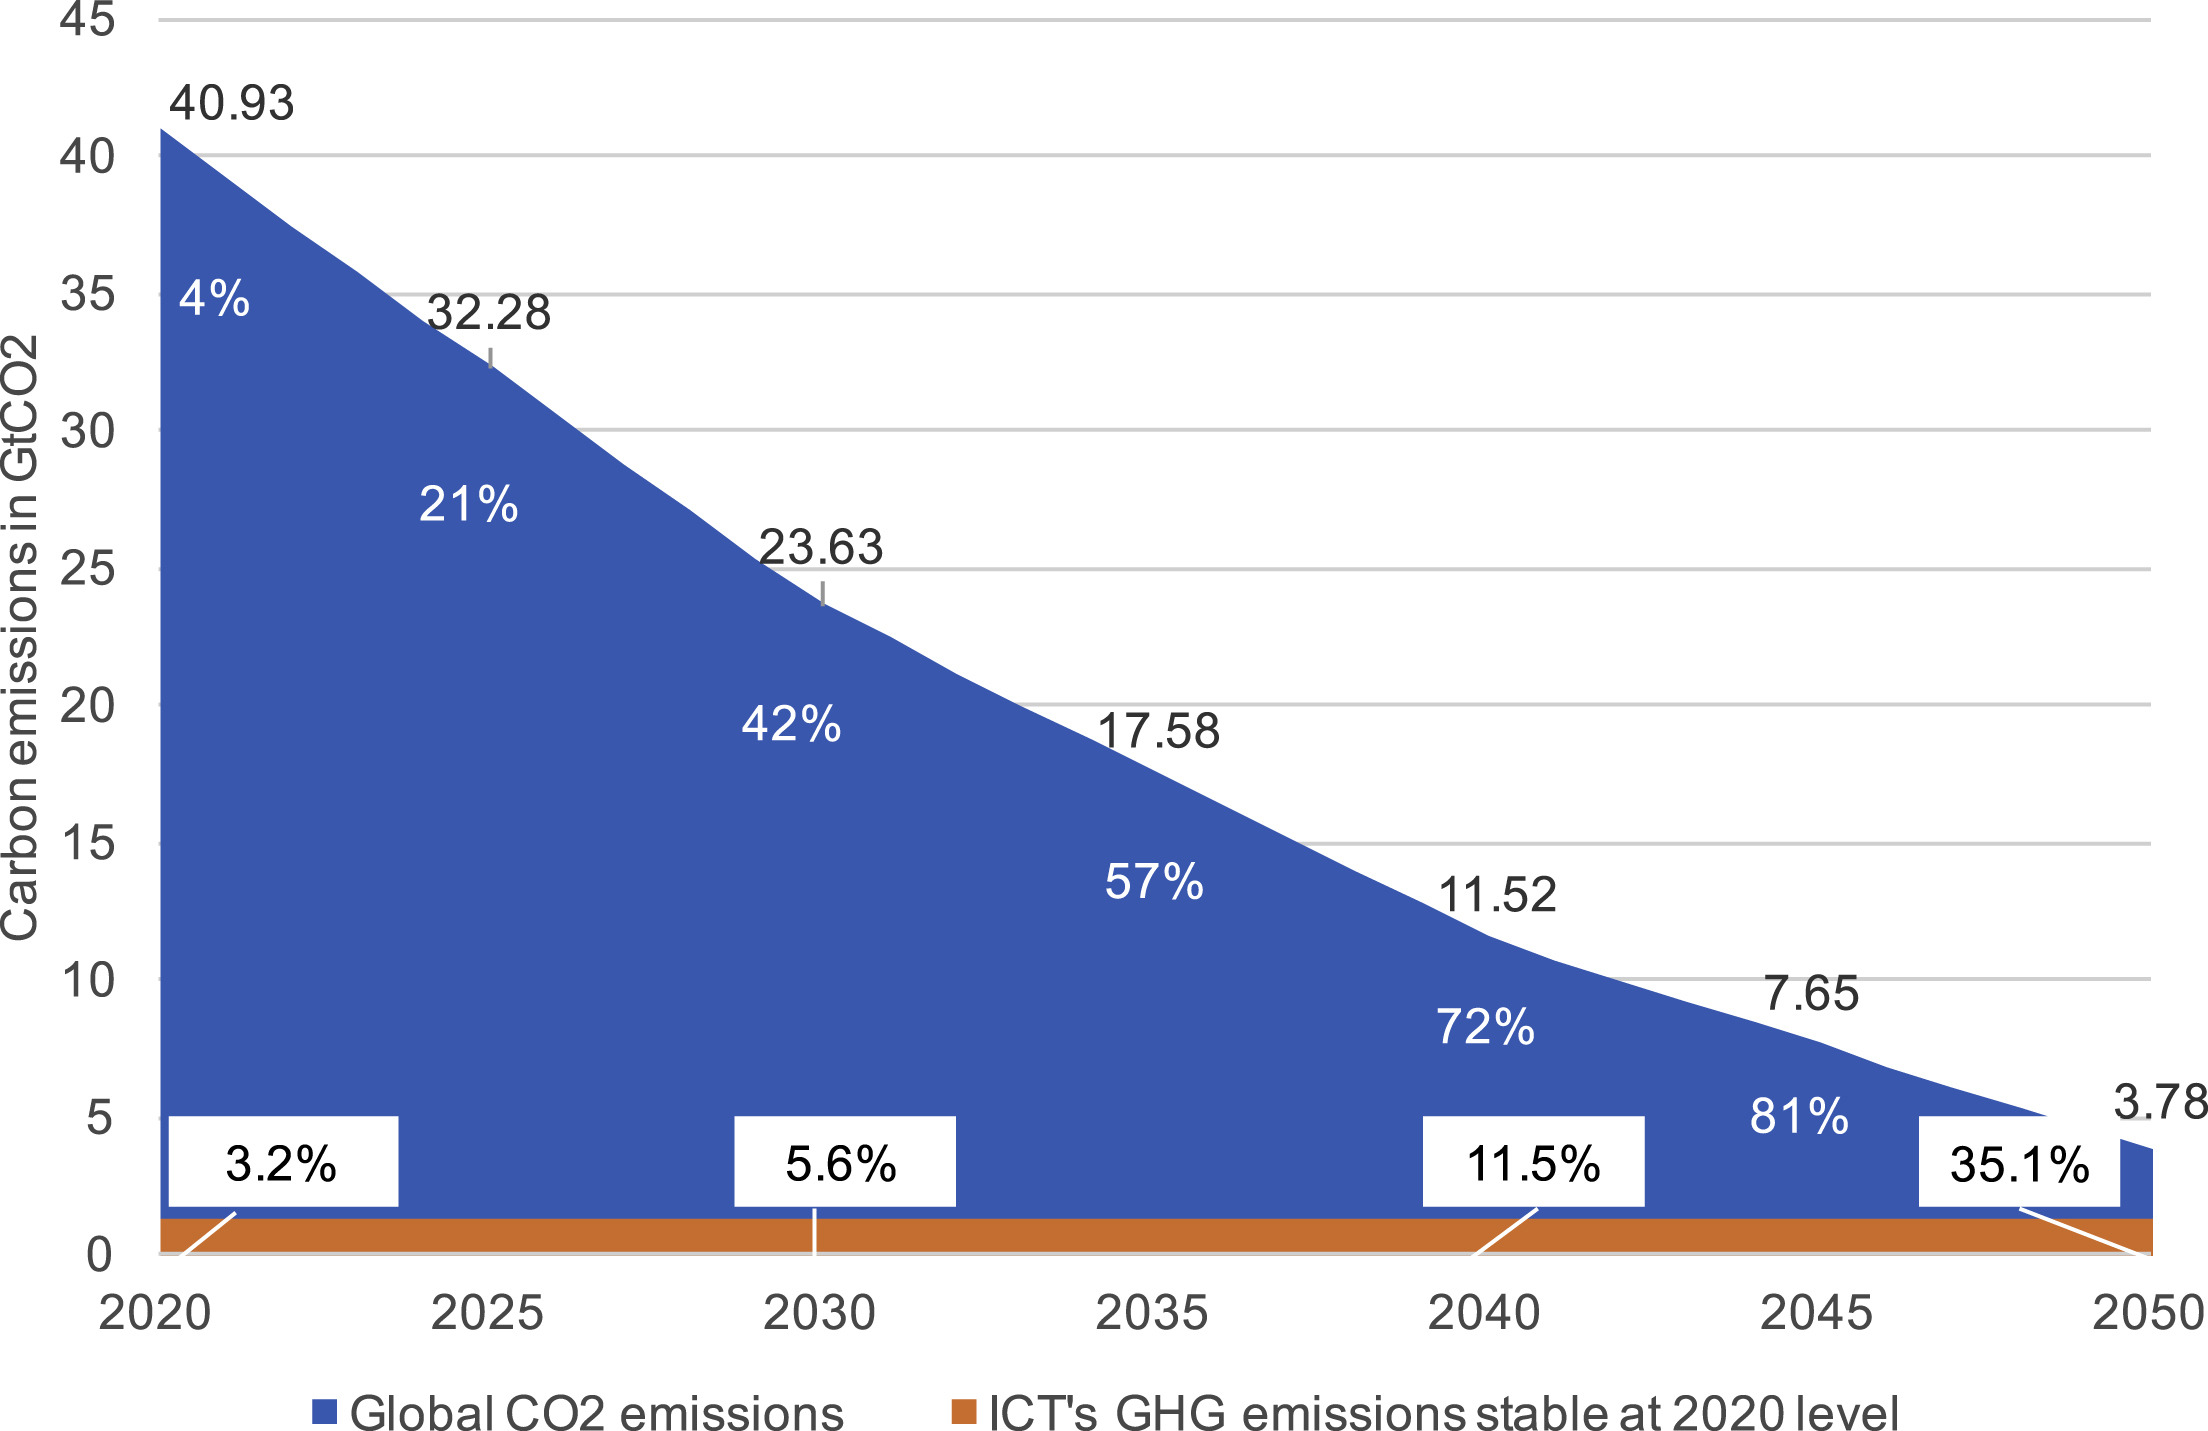
\includegraphics[scale=0.8]{Images/Related_works/gr6_lrg.jpg}
    \caption{ICT's emissions, assuming the 2020 level remains stable until 2050, and global CO2 emissions reduced in line with 1.5\degree C \cite{freitag2021climate}.}
    \label{fig:stable_emissions_ICT}
\end{figure}

\begin{figure}[!htb]
    \centering
    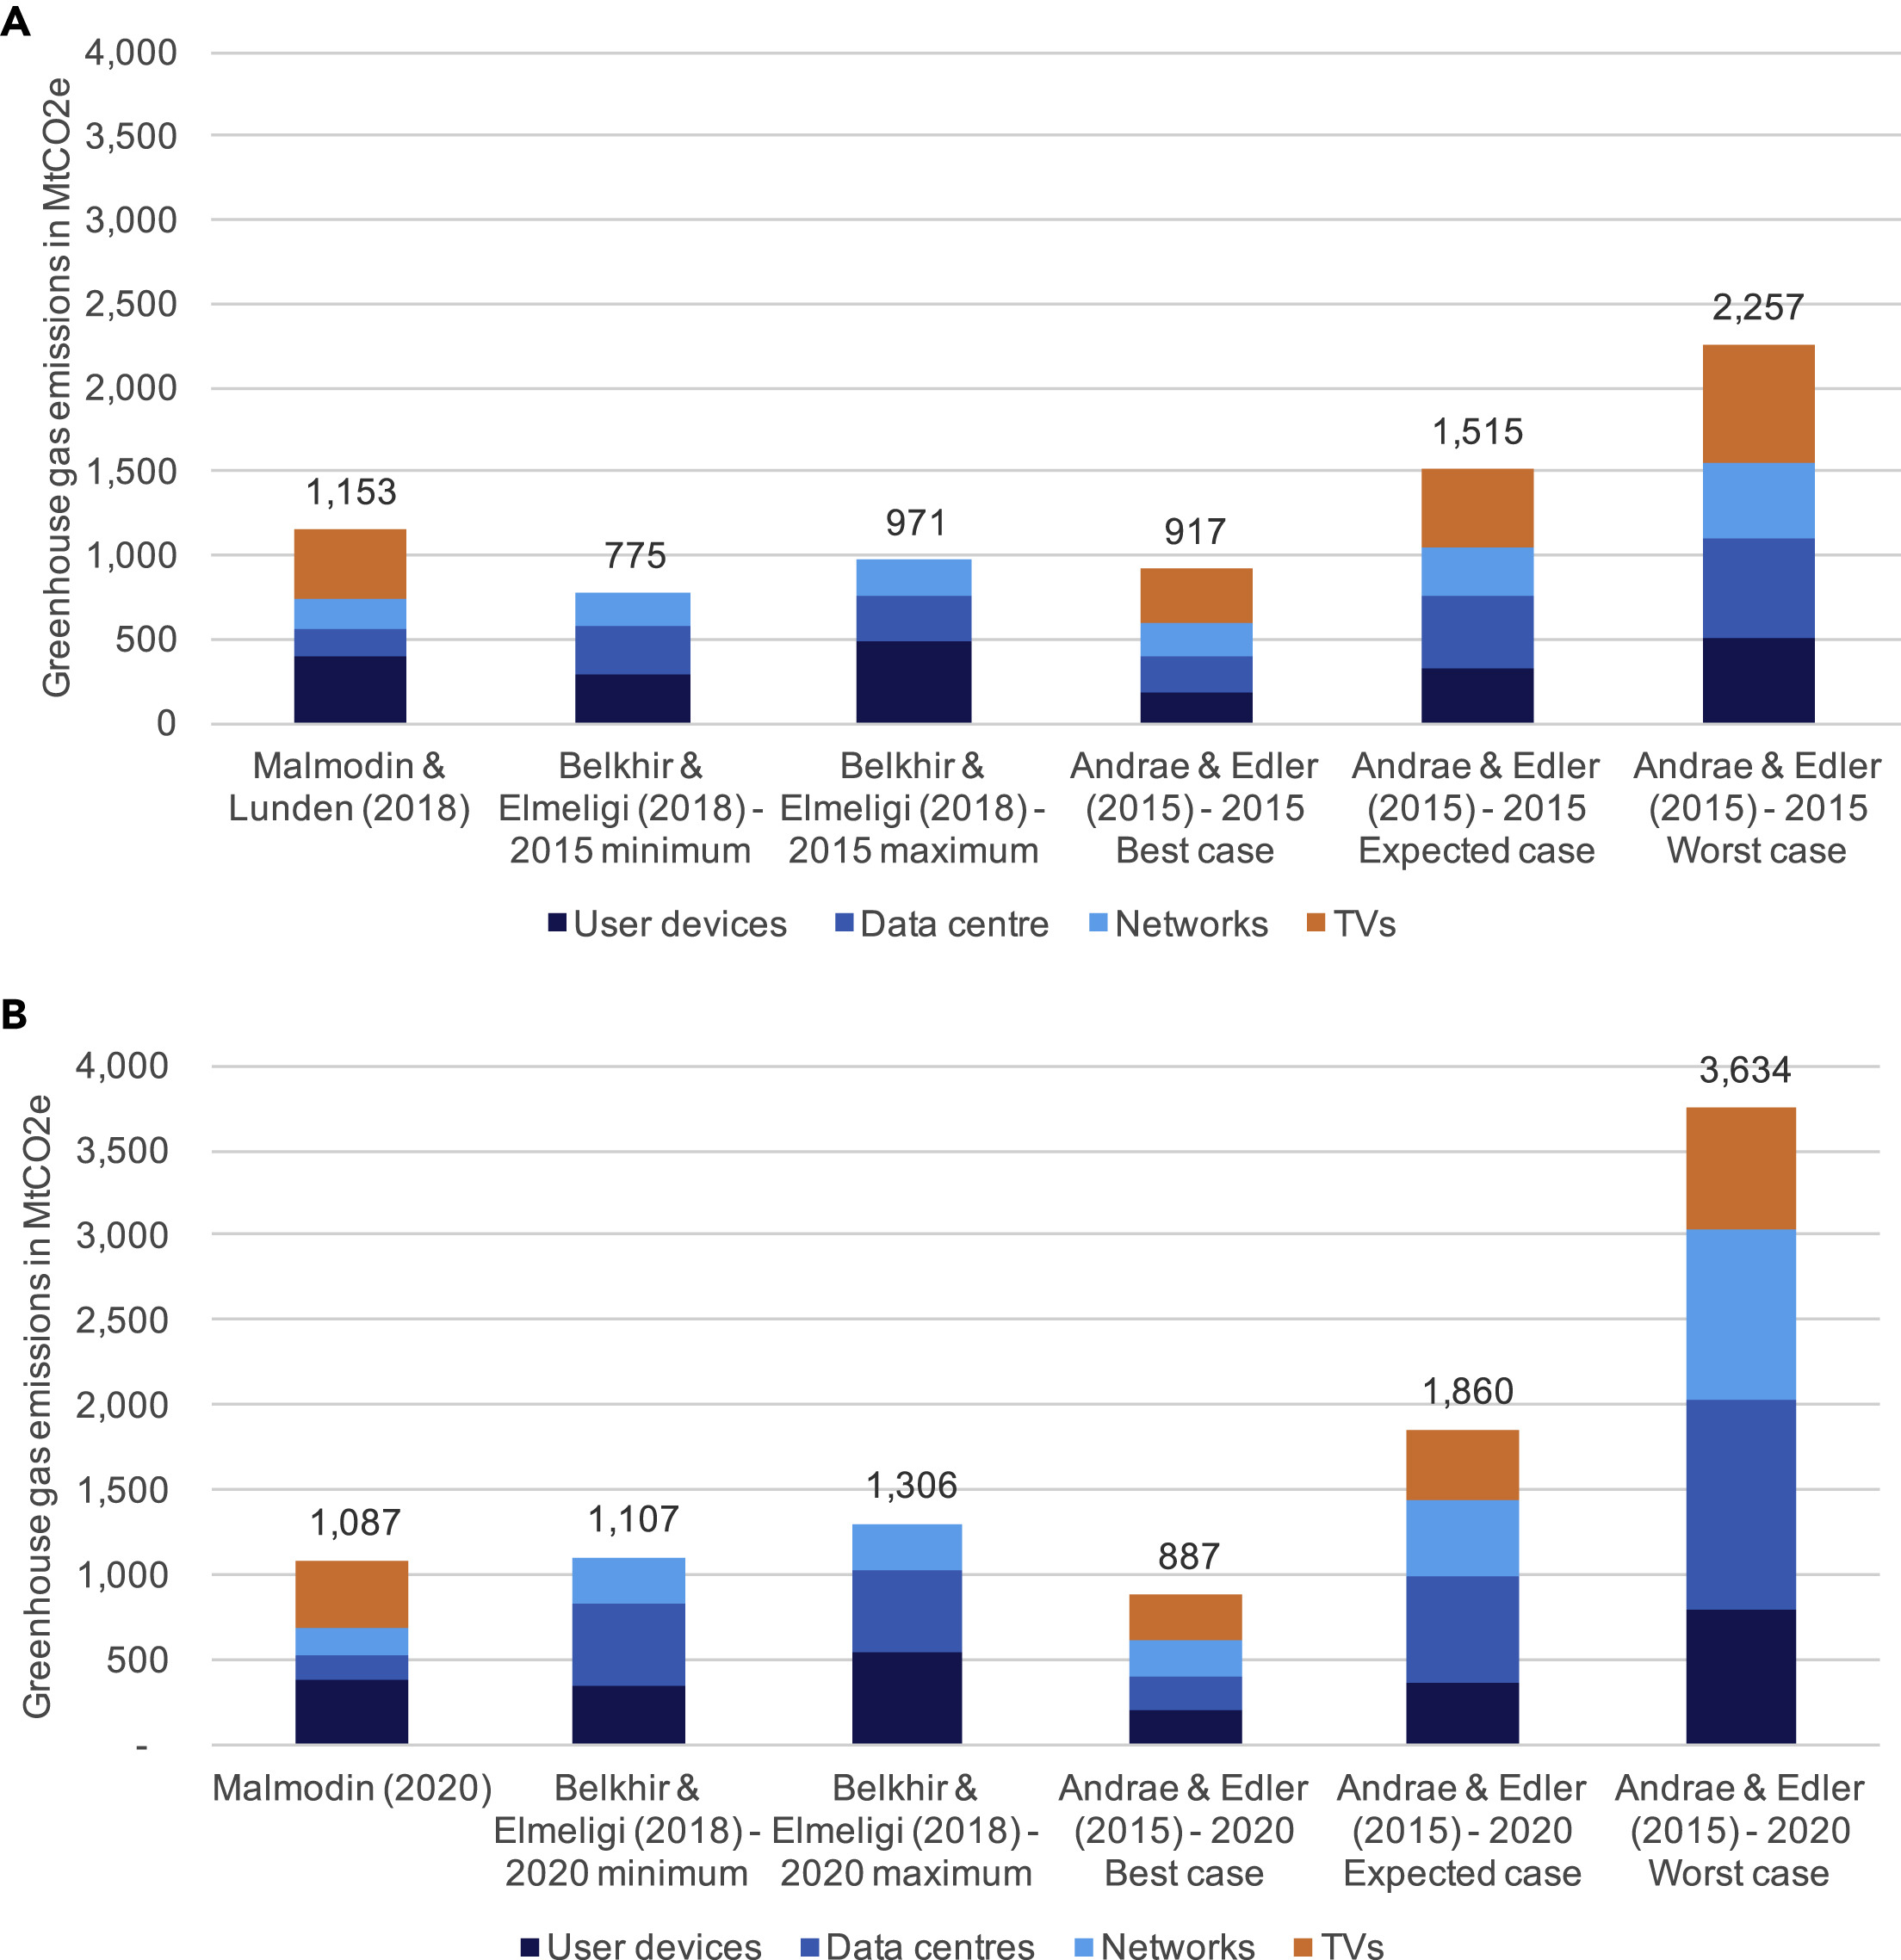
\includegraphics[scale=0.8]{Images/Related_works/gr2_lrg.jpg}
    \caption{Estimations for global ICT’s GHG emissions in 2015 and 2020 \cite{freitag2021climate}. The authors consolidated the works from \cite{belkhir2018assessing, andrae2015global, malmodin2018energy, Malmodin2020}.}
    \label{fig:estimations_ICT}
\end{figure}

Data centers are very energy consumers. IEA published an article indicating that data centers and networks were responsible for almost 1\% of energy-related GHG emissions in 2020 \cite{centres2022data}. Also, Google data centers consumed the same amount of energy as the entire city of San Francisco in 2015 \cite{khan2018exploiting}. Global data center electricity use in 2021 was 220-320 TWh, corresponding to 0.9-1.3\% of the global demand \cite{centres2022data}. For example, the domestic electricity consumption of Italy was 300 TWh in 2021 \cite{ElectricityDomesticConsumption}. In Ireland, electricity consumed by data centers went from 5\% of the total electricity consumption in 2015 to 14\% in 2021 \cite{IrelandDatacenter}. Denmark predicts to triple data center consumption, corresponding to 7\% of the country’s electricity use \cite{DenmarkDatacenter}.

Despite the strong growth in demand, data center energy usage has only moderately grown \cite{centres2022data}. A reason that explains it is the improvements in IT hardware energy consumption \cite{centres2022data}. These improvements allowed a boost in microchips' speed with a reduction in their power consumption, letting big data center companies cope with the peak in demand. Gordon Moore predicted in 1965 (Moore's law) that \cite{moore1965cramming}:

\begin{quote}
    ``The complexity for minimum component costs has increased at a rate of roughly a factor of two per year. Certainly over the short term this rate can be expected to continue, if not to increase. Over the longer term, the rate of increase is a bit more uncertain, although there is no reason to believe it will not remain nearly constant for at least 10 years.''
\end{quote}

Even if he predicted it just until 1975, it is the case nowadays. However, the future is uncertain, and the community is divided to confirm continuous efficiency improvements \cite{freitag2021climate}. While Andrae and Edler \cite{andrae2015global} and Belkhir and Elmeligi \cite{belkhir2018assessing} expected an ending in power-consuming improvements (indicated in Figure \ref{fig:projections_ICT}), Malmodin and Lundén \cite{malmodin2018energy} are more optimistic. They suggest that ICT’s carbon footprint in 2020 could halve by 2030. To achieve that, he considers two key factors. First, the improvements will continue. Second, the migration to renewable sources.

% \begin{itemize}
%     \item Present the numbers of global warming generally;
%     \item Present the predictions about the global warming;
%     \item Introduce the role of ICT generally;
%     \item Write about data center impact;
% \end{itemize}

\section{Renewable Energy Sources}

The ICT migration to renewable energy sources (RES) is one of the factors that helped reduce the growth in GHG emissions despite the rapidly growing demand for digital services \cite{centres2022data}. RES is one of the principal solutions to decarbonize electrical production \cite{olabi2022renewable, rostirolla2022survey}. RES is also named green energy, in contrast to brown energy from fossil fuels. Basically, RES generates energy from natural sources, such as solar, wind, geothermal, hydropower, wave and tidal, and biomass \cite{augustine2012renewable, panwar2011role, rostirolla2022survey, UNREnewable, gross2003progress}. These natural sources have a low impact on GHG emissions. For example, manufacturing is the stage with higher emissions for wind and solar \cite{amponsah2014greenhouse}. So, these components could produce energy with no or low GHG emissions. The renewable term comes from the idea that these sources are constantly replenished. On the other hand, fossil fuels are non-renewable because they need hundreds of millions of years to develop. In the Net Zero Emissions by 2050 Scenario, RES is responsible for one-third of the reductions between 2020 and 2030 \cite{renewables2022}. Some countries focus on nuclear power plants to produce energy \cite{kunsch2014nuclear}. Even if nuclear power is a low carbon emissions energy source, it introduces the risk of accidents and environmental impacts of radioactive wastes \cite{kunsch2014nuclear}.

The biggest challenge of implementing RES is its intermittence \cite{rostirolla2022survey}. Since RES production comes from nature, it depends on the climate conditions. For example, there is no power production from solar during the night. There are two approaches to reducing brown usage: on-site and off-site generation \cite{ren2012carbon}. On-site generation uses local renewable resources, and off-site takes resources available on the grid. In an off-site generation, it is not possible to guarantee that the incoming energy is from RES since the grid mixes all types of power generation \cite{rostirolla2022survey}. Giant cloud providers (e.g., Google, Amazon, and Facebook) invest in solar and wind power plants in an off-site approach \cite{Masanet984, branscombe2020google, amazon2023}. So, they could say that, on average, they provide RES to the grid with the same amount that they expend. However, they transfer the RES uncertainty problem to third parties \cite{rostirolla2022survey}. For example, in a case with a peak in demand, they will use the power from the grid, renewable or not. So, they are still non-renewable-dependent.

\section{Renewable-only Data center}
Since data centers have a controlled infrastructure, they are a good target to migrate to a renewable-only environment \cite{rostirolla2022survey}. However, creating a non-renewable independent data center imposes several challenges. In this kind of data center, all the generation is on-site without backup from the grid. Nevertheless, the production and demand can not match. Figure \ref{fig:load_production} exemplifies the mismatch between the power demanded by a data center and power generation. This mismatch requires a production (electrical) or a load (IT) shift. We will present both electrical and IT elements needed for a renewable-only data center.

\begin{figure}[!htb]
    \centering
    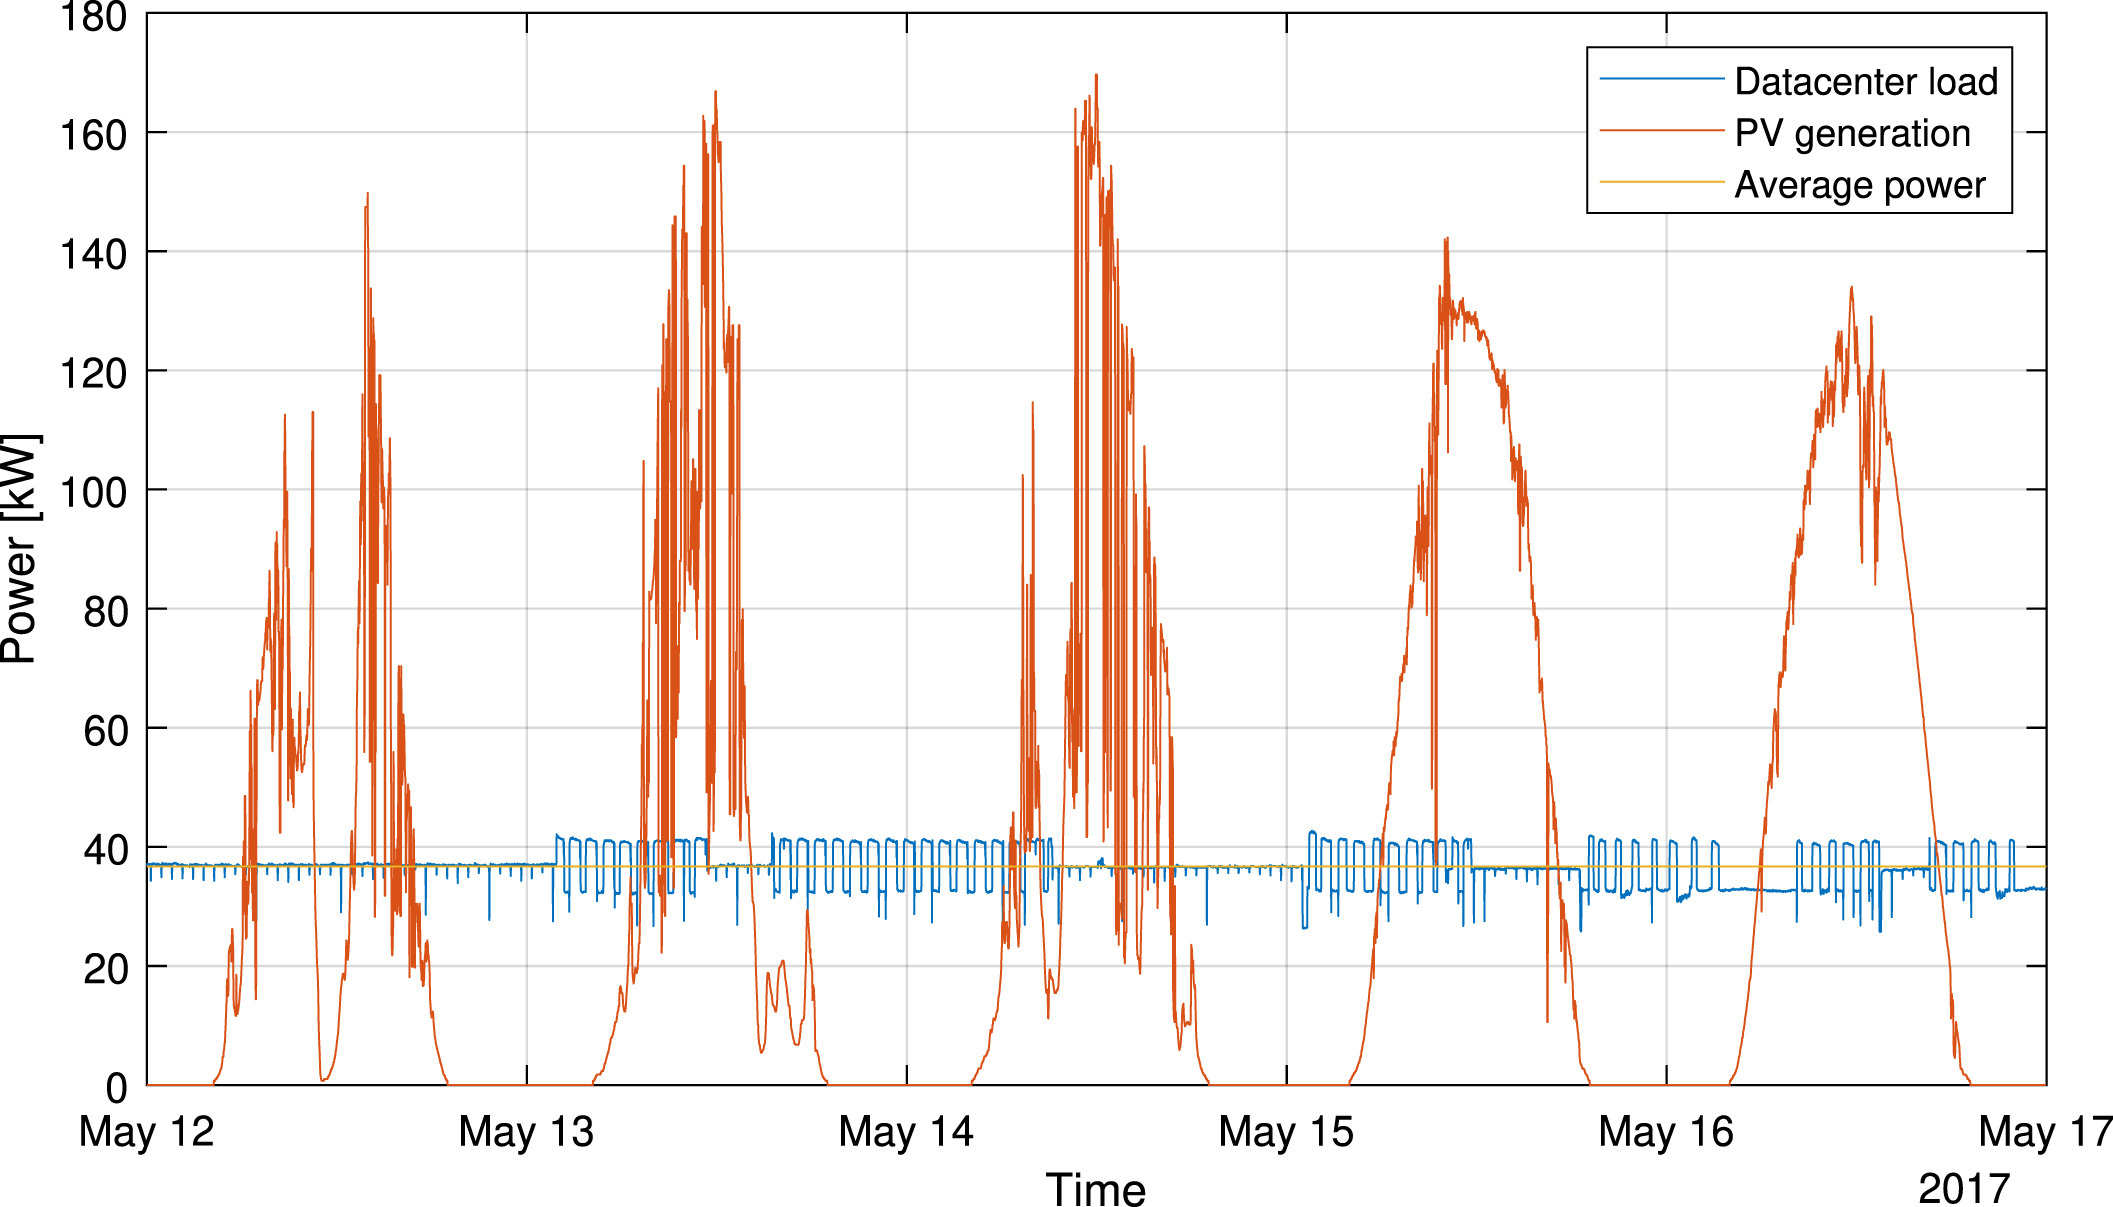
\includegraphics[scale=1]{Images/Related_works/load_production.jpg}
    \caption{Comparison of small data center load and the generation from a theoretical photovoltaic in Belfort, France. Both load and production have the same average value \cite{rostirolla2022survey}.}
    \label{fig:load_production}
\end{figure}

% \begin{itemize}
%     \item Explain the possibility of applying renewable in data centers;
%     \item Present the challenges in a renewable-only data center;
% \end{itemize}

\subsection{Electrical elements}
As mentioned before, different renewable sources can generate power. We focus on wind and solar since they were the most prominent in the past few years \cite{renewables2022}. For wind turbines, the wind speed is crucial. Equation \ref{equ:wind_turbines} gives the power output $P_{WT}(t)$ of a wind turbine, given the wind speed $v$ \cite{garcia2006wind, dong2016optimal, maleki2015optimal}.

\begin{equation}
    \label{equ:wind_turbines}
    P_{WT}(t) = \begin{cases}
        0 & v \leq v_{in} \text{ or } v(t) > v_{out} \\
        P_{WT,rated} \times \frac{v(t) - v_{in}}{v_{rated} - v_{in}} & v_{in} < v(t) \leq v_{rated} \\
        P_{WT,rated} & v_{rated} < v(t) \leq v_{out}
    \end{cases}
\end{equation}

Where:
\begin{itemize}
    \item $P_{WT}(t)$: Power generated by a wind turbine (kW);
    \item $v$: Wind speed (m/s);
    \item $v_{in}$: Cut-in wind speed (m/s);
    \item $v_{out}$: Cut-out wind speed (m/s);
    \item $v_{rated}$: Speed related to wind turbine nominal power (m/s);
    \item $P_{WT,rated}$: Wind turbine nominal power (kW).
\end{itemize}

If the wind speed $v$ is lesser or equal to the cut-in $v_{in}$  or greater than the cut-out $v_{out}$, it does not produce power. It tests the cut-out $v_{out}$ to protect the generator. If the speed $v$ is greater than the cut-in $v_{in}$ and lesser or equal to the rated speed $v_{rated}$, it generates proportionally to the rated power $P_{WT,rated}$ and rated speed $v_{rated}$. Finally, if the speed $v$ is greater than the rated speed $v_{rated}$ and lesser or equal to the cut-out $v_{out}$, it produces constant power $P_{WT,rated}$. 

Regarding solar production, the photovoltaic (PV) system uses solar panels to generate power from solar irradiation. Equation \ref{equ:panel_solar_with_temperature} demonstrates how to calculate the output power of a solar panel $P_{pv}(t)$ \cite{maleki2015optimal, sinha2015review, dong2016optimal}.

\begin{equation}
    \label{equ:panel_solar_with_temperature}
    P_{pv}(t) = P_{R,PV} \times (R / R_{ref}) \times \eta_{PV}
\end{equation}

Where:
\begin{itemize}
    \item $P_{pv}(t)$: Power generated by each PV panel (W);
    \item $P_{R,PV}$: PV panel Nominal power (kW);
    \item $R$: Solar radiation (W/$m^{2}$);
    \item $R_{ref}$: solar radiation at reference conditions. Usually set as 1000 (W/$m^{2}$) \cite{dong2016optimal};
    \item $\eta_{PV}$: PV efficiency.
\end{itemize}

Regarding PV efficiency $\eta_{PV}$, it can consider the temperature of the solar panel \cite{sinha2015review, maleki2015optimal}. However, some works simplify it by applying a constant value \cite{dong2016optimal, haddad2019mixed}. 

% \begin{itemize}
%     \item Write about wind turbines;
%     \item Write about solar panel;
%     \item Write about battery;
%     \item Write about Electrolyzer;
%     \item Write about Fuel Cell;
%     \item Write about hydrogen;
% \end{itemize}

\subsection{IT elements}
\begin{itemize}
    \item Write about the servers;
    \item Write about the power consumption (e.g., DVFS, on-off, idle, etc);
    \item Write about the jobs (e.g., types, resources demanded, etc);
\end{itemize}

\section{Sources of Uncertainty}

\subsection{Weather Uncertainties}
\begin{itemize}
    \item Describe wind uncertainty;
    \item Describe solar irradiation uncertainty;
\end{itemize}

\subsection{Workload Uncertainties}
\begin{itemize}
    \item Describe job arrival uncertainty;
    \item Describe job size uncertainty;
\end{itemize}

\section{Optimization Strategies for Dealing with Uncertainties}
\begin{itemize}
    \item Write about weather predictions
    \item Write about optimization for the weather;
    \item Write about scheduling algorithms to deal with workload uncertainties;
    \item Write about mixing both renewable production and workload uncertainties;
\end{itemize}

\section{Literature Review}

\begin{itemize}
    \item Present the 20 articles selected;
    \item Present a table with each article and the following points:
    \begin{itemize}
        \item Name;
        \item Year;
        \item Source of power (solar, wind, battery, grid, etc);
        \item Level of decision (offline, online, both);
        \item Power adaptations (battery compensations, renewable adaptations, etc).
    \end{itemize}
\end{itemize}

\subsection{Discussion and Classification of the Literature}